\documentclass[10pt,french]{book}

\input philippe2013

\pagestyle{empty}

\begin{document}
\vspace*{-2cm}

\begin{center}
\renewcommand\arraystretch{2.5}
    \begin{tabular}{*{10}{|>{\centering\arraybackslash}m{1cm}}|}
        \hline
            $x$ & $0$ & $\frac{\pi}{6}$ & $\frac{\pi}{4}$ & $\frac{\pi}{3}$ & $\frac{\pi}{2}$ & $\pi$ & $\frac{5\pi}{4}$ & $\frac{3\pi}{2}$ & $2\pi$\\
        \hline
            $\cos x$ & &&&&&&&&\\
        \hline
            $\sin x$&&&&&&&&& \\
        \hline
    \end{tabular}
\end{center}

\begin{center}
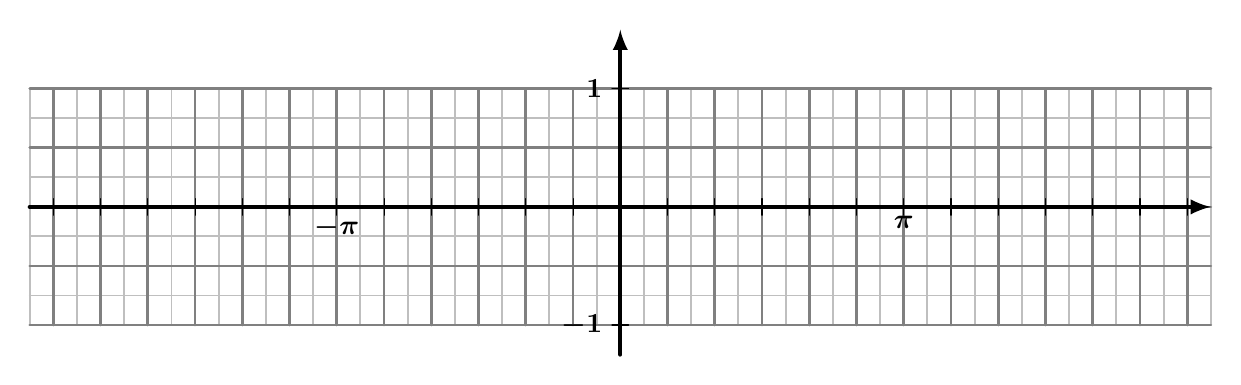
\begin{tikzpicture}[line cap=round,line join=round,>=latex,y=1.5cm,x=0.6cm]
\draw [color=gray!50, xstep=0.5,ystep=0.25,line width=0.7pt] (-12.5,-1) grid (12.5,1);
\draw [color=gray,xstep=1.0,ystep=0.5,line width=1pt,] (-12.5,-1) grid (12.5,1);
\draw[->,line width=1.5pt] (-12.5,0) -- (12.5,0);
\foreach \x in {-12,...,12}
\draw[color=black] (\x,3pt) -- (\x,-3pt);
\draw[->,line width=1.5pt] (0,-1.25) -- (0,1.5);
\foreach \y in {-1,1}
\draw[color=black] (3pt,\y) -- (-3pt,\y) node[left,font=\boldmath] {$\y$};
\draw (-6,0) node[below,font=\boldmath] {$-\pi$};
\draw (6,0) node[below,font=\boldmath] {$\pi$};
\end{tikzpicture}
\end{center}\bigskip

\noindent\dotfill\bigskip

\begin{center}
\renewcommand\arraystretch{2.5}
    \begin{tabular}{*{10}{|>{\centering\arraybackslash}m{1cm}}|}
        \hline
            $x$ & $0$ & $\frac{\pi}{6}$ & $\frac{\pi}{4}$ & $\frac{\pi}{3}$ & $\frac{\pi}{2}$ & $\pi$ & $\frac{5\pi}{4}$ & $\frac{3\pi}{2}$ & $2\pi$\\
        \hline
            $\cos x$ & &&&&&&&&\\
        \hline
            $\sin x$&&&&&&&&& \\
        \hline
    \end{tabular}
\end{center}

\begin{center}
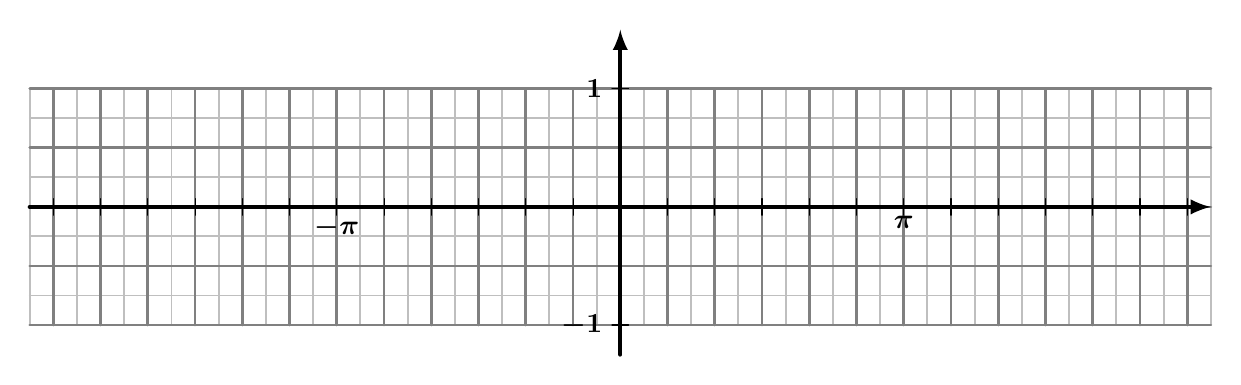
\begin{tikzpicture}[line cap=round,line join=round,>=latex,y=1.5cm,x=0.6cm]
\draw [color=gray!50, xstep=0.5,ystep=0.25,line width=0.7pt] (-12.5,-1) grid (12.5,1);
\draw [color=gray,xstep=1.0,ystep=0.5,line width=1pt,] (-12.5,-1) grid (12.5,1);
\draw[->,line width=1.5pt] (-12.5,0) -- (12.5,0);
\foreach \x in {-12,...,12}
\draw[color=black] (\x,3pt) -- (\x,-3pt);
\draw[->,line width=1.5pt] (0,-1.25) -- (0,1.5);
\foreach \y in {-1,1}
\draw[color=black] (3pt,\y) -- (-3pt,\y) node[left,font=\boldmath] {$\y$};
\draw (-6,0) node[below,font=\boldmath] {$-\pi$};
\draw (6,0) node[below,font=\boldmath] {$\pi$};
\end{tikzpicture}
\end{center}\bigskip

\noindent\dotfill\bigskip

\begin{center}
\renewcommand\arraystretch{2.5}
    \begin{tabular}{*{10}{|>{\centering\arraybackslash}m{1cm}}|}
        \hline
            $x$ & $0$ & $\frac{\pi}{6}$ & $\frac{\pi}{4}$ & $\frac{\pi}{3}$ & $\frac{\pi}{2}$ & $\pi$ & $\frac{5\pi}{4}$ & $\frac{3\pi}{2}$ & $2\pi$\\
        \hline
            $\cos x$ & &&&&&&&&\\
        \hline
            $\sin x$&&&&&&&&& \\
        \hline
    \end{tabular}
\end{center}

\begin{center}
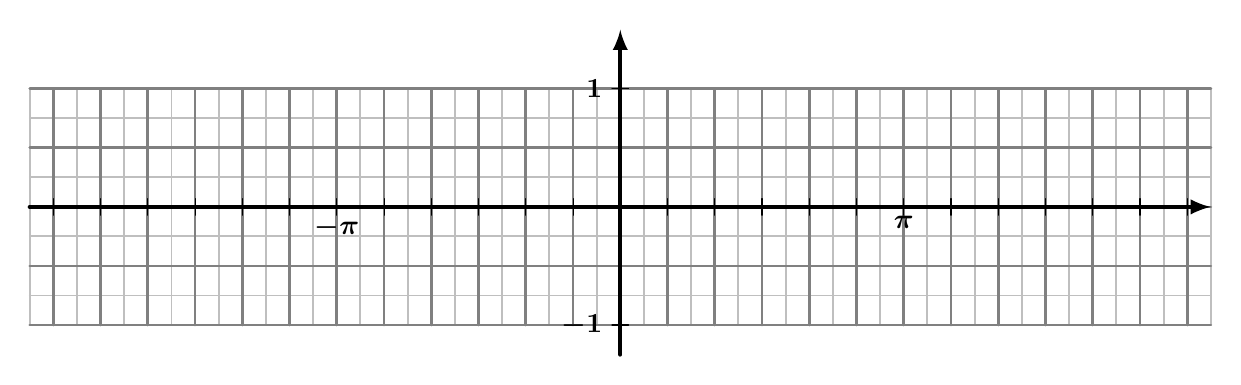
\begin{tikzpicture}[line cap=round,line join=round,>=latex,y=1.5cm,x=0.6cm]
\draw [color=gray!50, xstep=0.5,ystep=0.25,line width=0.7pt] (-12.5,-1) grid (12.5,1);
\draw [color=gray,xstep=1.0,ystep=0.5,line width=1pt,] (-12.5,-1) grid (12.5,1);
\draw[->,line width=1.5pt] (-12.5,0) -- (12.5,0);
\foreach \x in {-12,...,12}
\draw[color=black] (\x,3pt) -- (\x,-3pt);
\draw[->,line width=1.5pt] (0,-1.25) -- (0,1.5);
\foreach \y in {-1,1}
\draw[color=black] (3pt,\y) -- (-3pt,\y) node[left,font=\boldmath] {$\y$};
\draw (-6,0) node[below,font=\boldmath] {$-\pi$};
\draw (6,0) node[below,font=\boldmath] {$\pi$};
\end{tikzpicture}
\end{center}


\end{document}